\documentclass{beamer}

\usetheme{Madrid}
\setbeamertemplate{navigation symbols}{}
\setbeamertemplate{caption}[numbered]


\usepackage{graphicx}
\usepackage{amsmath}
%\usepackage{xeCJK}
\usepackage{booktabs}
\usepackage{multirow}
\usepackage{tikz}
\usepackage{makecell}


\title[Democratic Peace Revisited]{The Theory of Democratic Peace Revisited \\ \large{Exogenous Regime or \textit{Pax Americana}}}
\author{Chen Zeng}
\institute[]{Department of Political Science \\ Renmin University of China}

\begin{document}
	\maketitle

	\begin{frame}{Introduction}
		\begin{figure}
			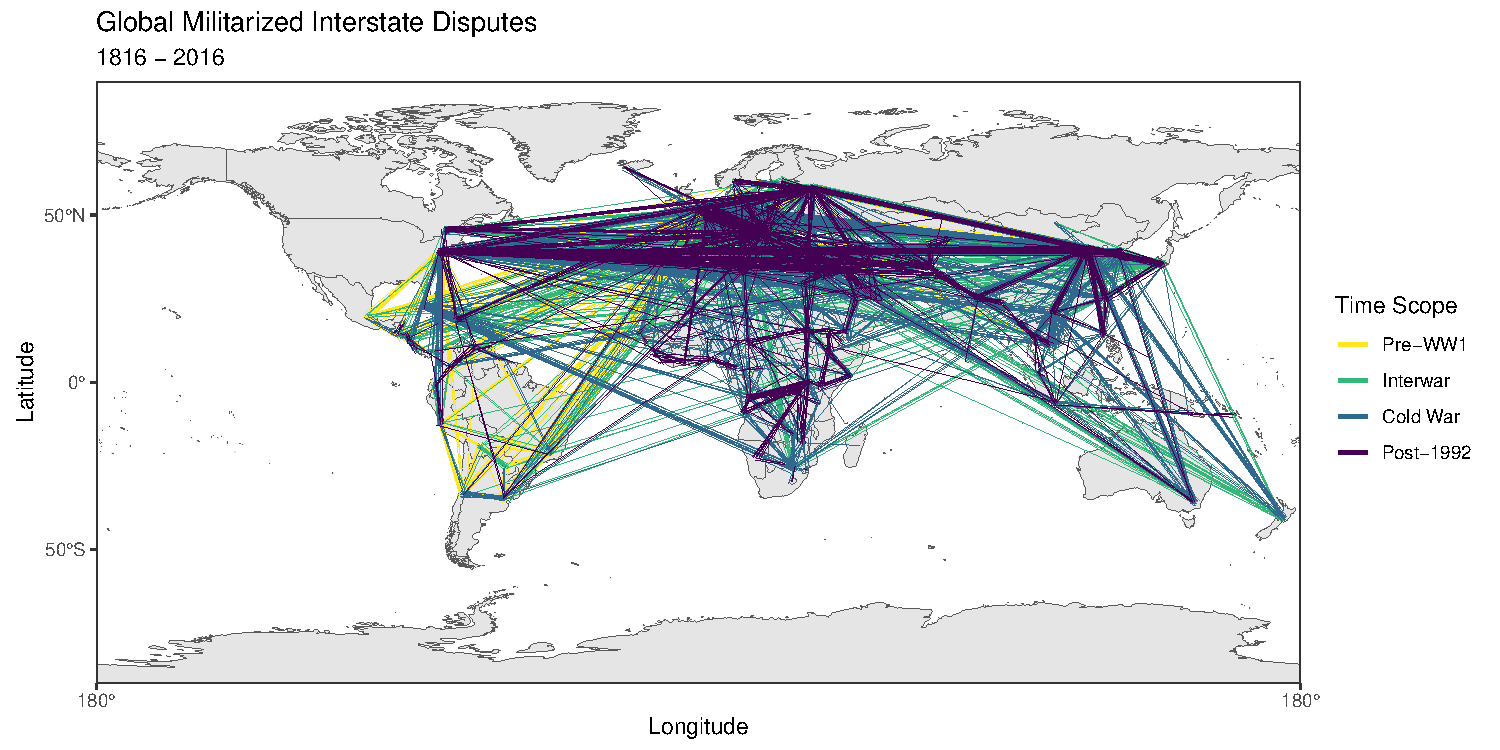
\includegraphics[width=\linewidth]{data/output/plots/all.pdf}
			\caption{Global MIDs Disaggregated by Time Periods (1816--2016)}
		\end{figure}
	\end{frame}
	
	\begin{frame}{Contents}
		\tableofcontents
	\end{frame}

	\section{Conceptualizing Democratic Peace}
	
	\subsection{Militarized Disputes, War, and Peace}
	
	\subsection{Democracy: Normative and Empirical}
	
	\subsection{Operationalizing Democratic Peace}

	\section{Forty Years of Empirical Democratic Peace Study}
	
	\subsection{Revival of the Democratic Peace Thesis}
	
	\subsection{Consolidation of Research Design Consensus}
	
	\subsection{Causal Mechanism of Democratic Peace}
	
	\subsection{Emergence of Alternative Theoretical Explanations}

	\section{Analysis}
	
	\subsection{Tracing the Mechanism of Democratic Peace}
	
	\subsection{Disaggregating the Democratic Peace}
	
	\subsection{Democratic Peace and Great Power Hierarchy}
	
	\section{Conclusion}
	
	hi
	
\end{document}